\section{ProtoDUNE-ND}
\label{sec:protodune-nd}
In this section, the technical design of the proposed ProtoDUNE-ND at Fermilab is described. First, a consideration of the available neutrino beamlines is carried out in Section~\ref{sec:neutrino-flux}, which shows that the on-axis medium-energy NuMI beam provides a rate closest to that of the future, intense, LBNF beamline~\cite{DUNE3}. Second, a discussion of the MINOS near detector hall is provided in Section~\ref{sec:minos-hall}, with consideration given to the existing and required infrastructure to support the ProtoDUNE-ND detectors. Then, a discussion of the technical aspects of each of the ProtoDUNE-ND detectors is given: the ArgonCube 2x2 Demonstrator module in Section~\ref{sec:2x2-design}; the 3DST demonstrator module in Section~\ref{sec:3dst-design}; and the HPTPC demonstrator in Section~\ref{sec:hptpc-design}. \todo{Modify as appropriate... if there's only ArgonCube information available, we can note the possibility of others being included, and comment on the branch points when decisions about whether to include them or not must be made.}

\subsection{Neutrino flux study}
\label{sec:neutrino-flux}
The LBNF beamline is an intense source of muon (anti-)neutrinos, with a much higher flux of neutrinos than accelerator neutrino beams currently in operation~\cite{DUNE3}. A key design requirement for the DUNE near detectors, and one of the primary concerns motivating the proposal to build ProtoDUNE-ND is how well the near detector components will perform in a high multiplicity environment. It is therefore worth asking how suitable existing beamlines are for providing a useful neutrino beam test for the proposed near detector components.

\begin{figure}[htb]
  \centering
  \subfloat[Flux\label{subfig:flux}]    {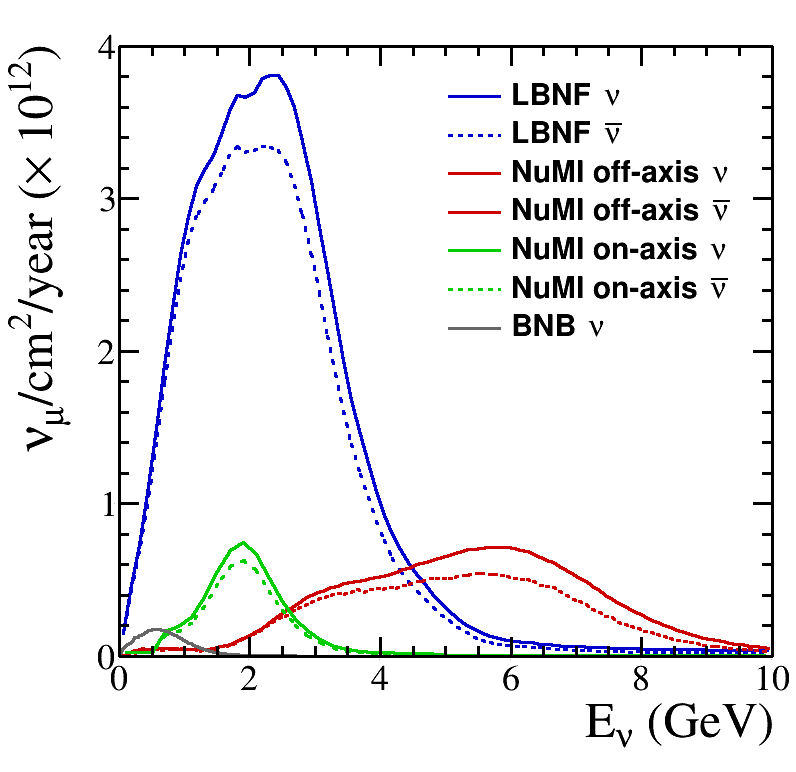
\includegraphics[width=0.5\textwidth]{plots/fnal_flux_comparison.png}}
  \subfloat[Rate\label{subfig:rate}]    {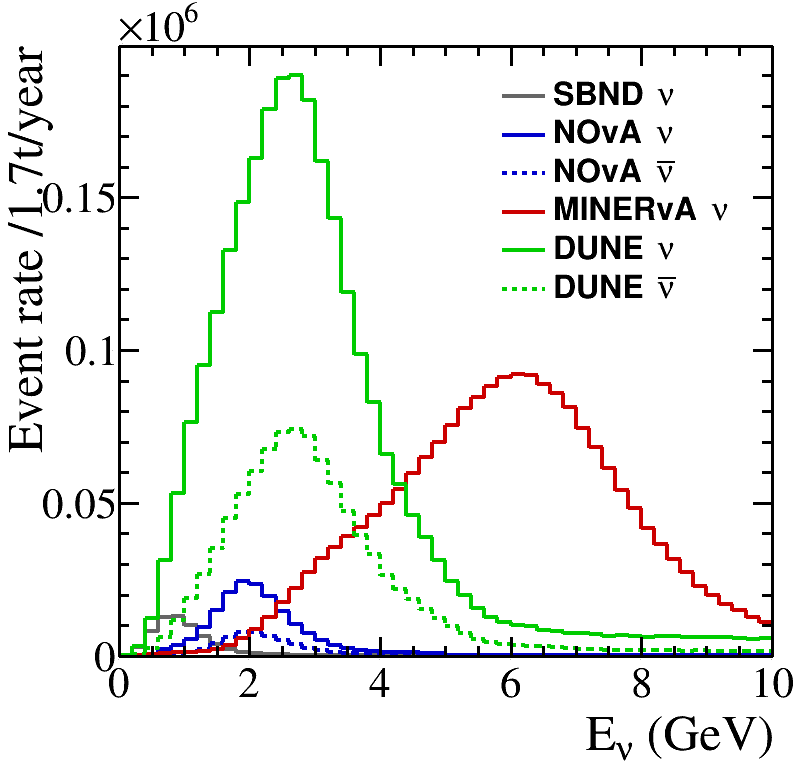
\includegraphics[width=0.5\textwidth]{plots/2x2_Enu_all.png}}
  \caption{Comparison of the absolutely normalized fluxes for different neutrino beamlines at Fermilab, and the expected yearly rates in a 1.7t LAr volume as a function of \enu, produced using GENIE v2.12.8 with the ``ValenciaQEBergerSehgalCOHRES'' configuration~\cite{genie}.}
  \label{fig:beam_options}
\end{figure}
In Figure~\ref{subfig:flux}, the currently available neutrino fluxes at various near detector halls in Fermilab are compared, on an absolutely normalized scale, to the LBNF three-horn optimized flux at the 574~m near detector site~\addcite. The currently available neutrino fluxes considered are the on- and 14 mrad. off-axis medium-energy neutrinos from the main injector (NuMI) beam~\cite{numi}, which corresponds to the MINOS and NOvA near detector halls; and the booster neutrino beam (BNB) at the SBND hall~\addcite. The FY2017 delivered POT was used to produce a yearly flux and rate for the BNB and NuMI beams~\cite{fnal_beam_2017}. It is clear that the proposed LBNF flux is significantly more intense than the fluxes sampled at any existing experimental hall. However, due to the roughly linear relationship between neutrino energy and cross section, the measured rate from the on-axis NuMI beam in the MINOS-ND hall is approximately the same, and is therefore the most desirable currently functional experimental hall at Fermilab for a ProtoDUNE-ND test. The rate has been produced with the GENIE neutrino interaction Monte Carlo package~\cite{genie}, using v2.12.8 with the ValenciaQEBergerSehgalCOHRES configuration. Note that the rate is normalized to the active volume of the ArgonCube 2x2 Demonstrator module, showing that significant statistics will be accumulated in a matter of months of ProtoDUNE-ND operation.

\FloatBarrier
\subsection{MINOS near detector hall}
\label{sec:minos-hall}
\begin{itemize}
\item Size of the hall
\item Existing infrastructure required for the test
\item Need to consider whether we need to move anything (e.g. MINERvA) to make space
\item New infrastructure to be put in for the test --> Barry Norris/ Alan Bross. Probably need to discuss language with Steve Brice to make it forceful enough
\end{itemize}

\subsection{ArgonCube 2x2 Demonstrator module}
\label{sec:2x2-design}

\todo{James, please fix this section!}
ArgonCube, and the Argoncube 2x2 Demonstrator module are described in Ref.~\cite{argoncube_loi}. However, a number of significant changes to the design have been made since then, to account for the advancements made in the ArgonCube R\&D program. In particular, the four modules of the ArgonCube 2x2 Demonstrator will not test separate technologies, as design choices have already been informed by smaller scale tests. Instead, the modules will be functionally identical, to allow for more sophisticated reconstruction tests.

\begin{figure}[htbp]
\centering
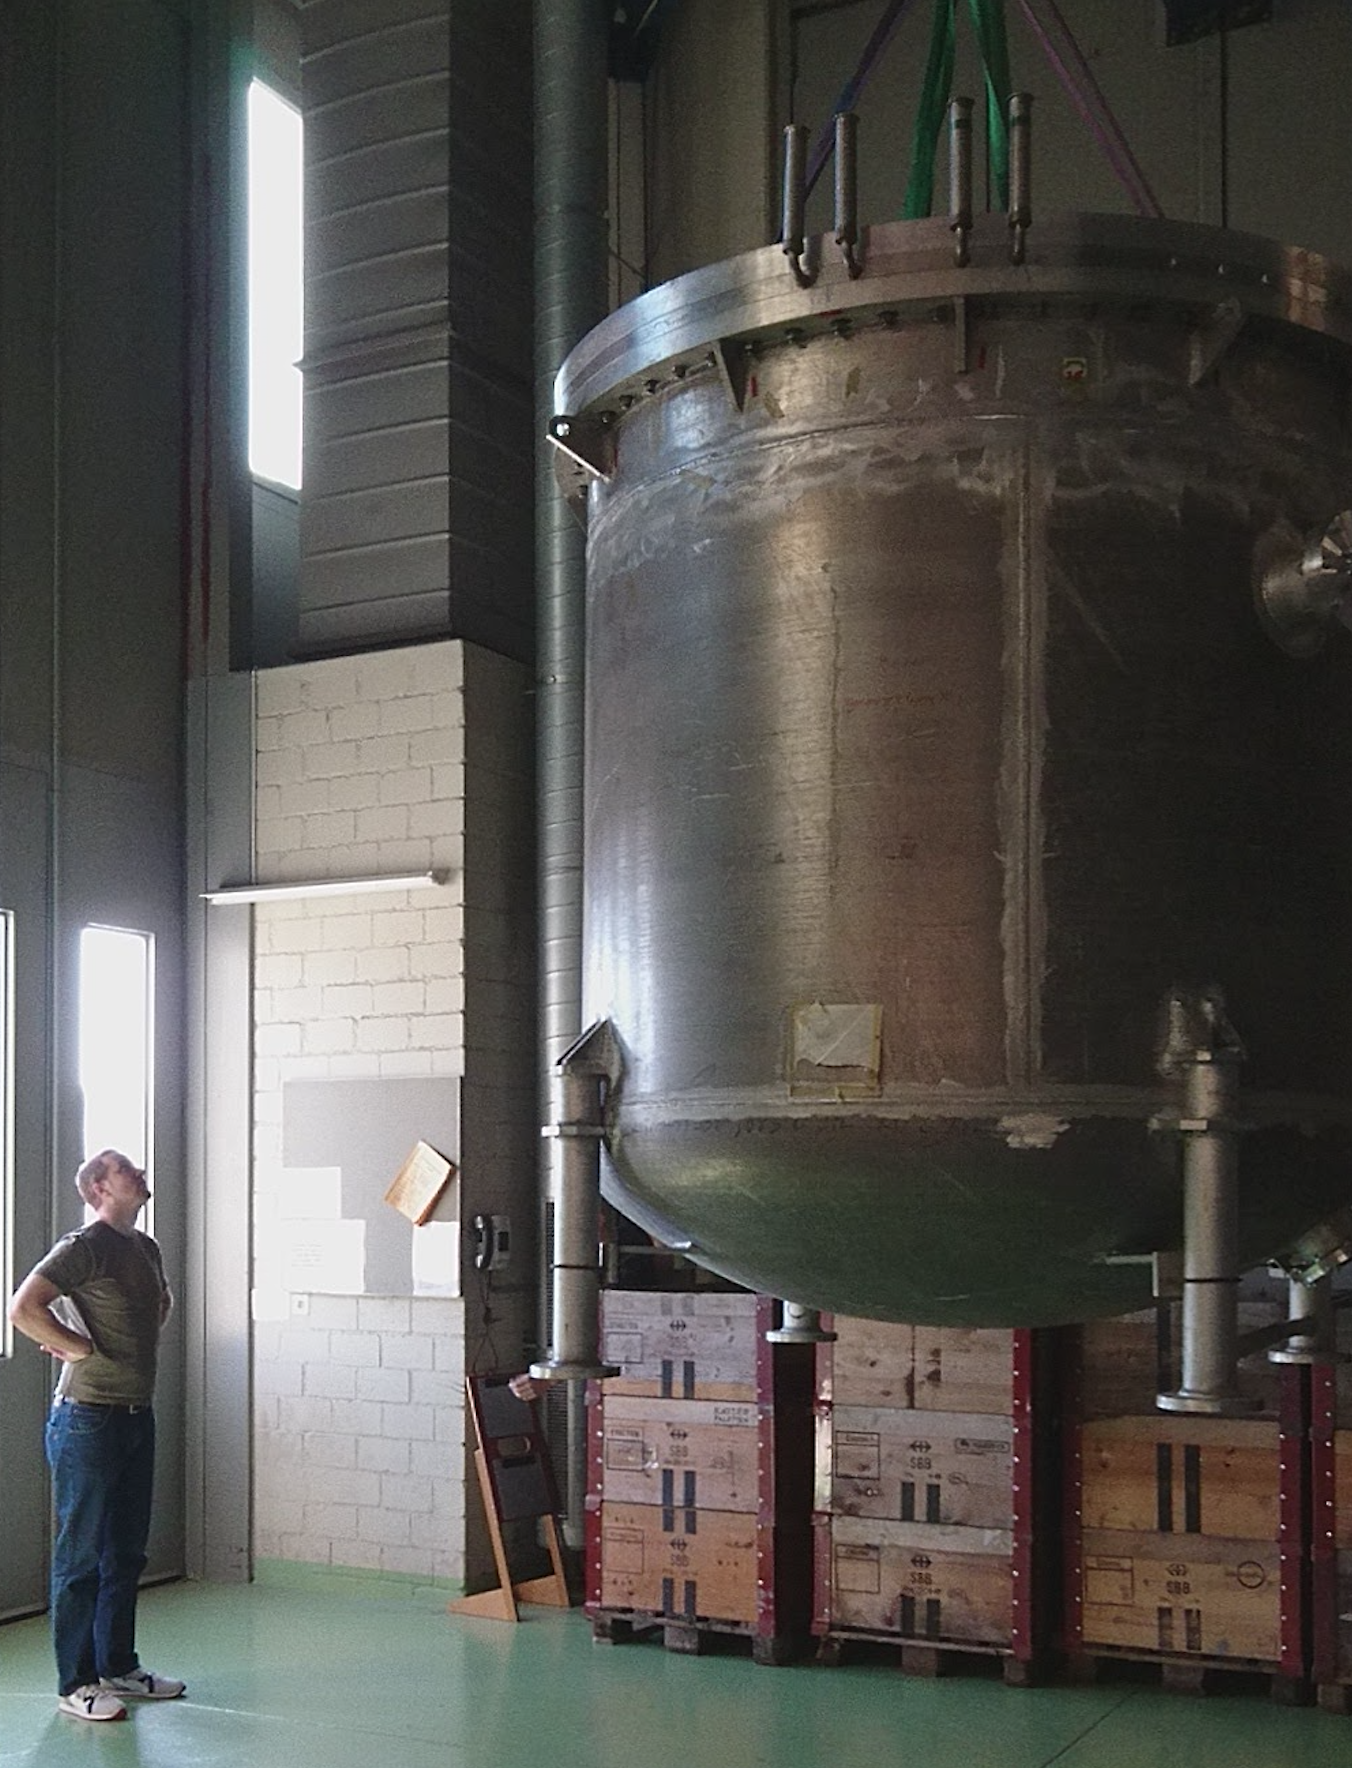
\includegraphics[width=0.45\linewidth]{plots/cryostat.png}
\caption{Cryostat that will host the ArgonCube 2x2 Demonstrator module, reproduced from Ref.~\cite{argoncube_loi}.}
\label{fig:2x2_cryostat}
\end{figure}
ArgonCube is made of self-contained TPC modules sharing a common cryostat. Each module is made of a rectangular box with a square footprint, and a height to be optimized in order to meet the physics goals and/or sensitivity constraints. The ArgonCube 2x2 Demonstrator module will be housed within an existing vacuum-insulated cryostat, shown in Figure~\ref{fig:2x2_cryostat}, which is $\sim$\SI{2.2}{\metre} in diameter, and $\sim$\SI{2.8}{\metre} deep, for a total volume of $\sim$6 m$^3$. The size of the cryostat sets the dimensions of the modules for the demonstrator. The square base of each module will be \SI{0.67 x 0.67}{\metre}, and the height will be \SI{1.81}{\metre}. This makes the modules comparable in size to, but slightly smaller than for the proposed DUNE near detector, which will have a base of \SI{1 x 1}{\metre}, with a height to be optimized in order to meet the physics goals and/or sensitivity constraints.

\begin{figure}[htbp]
\centering
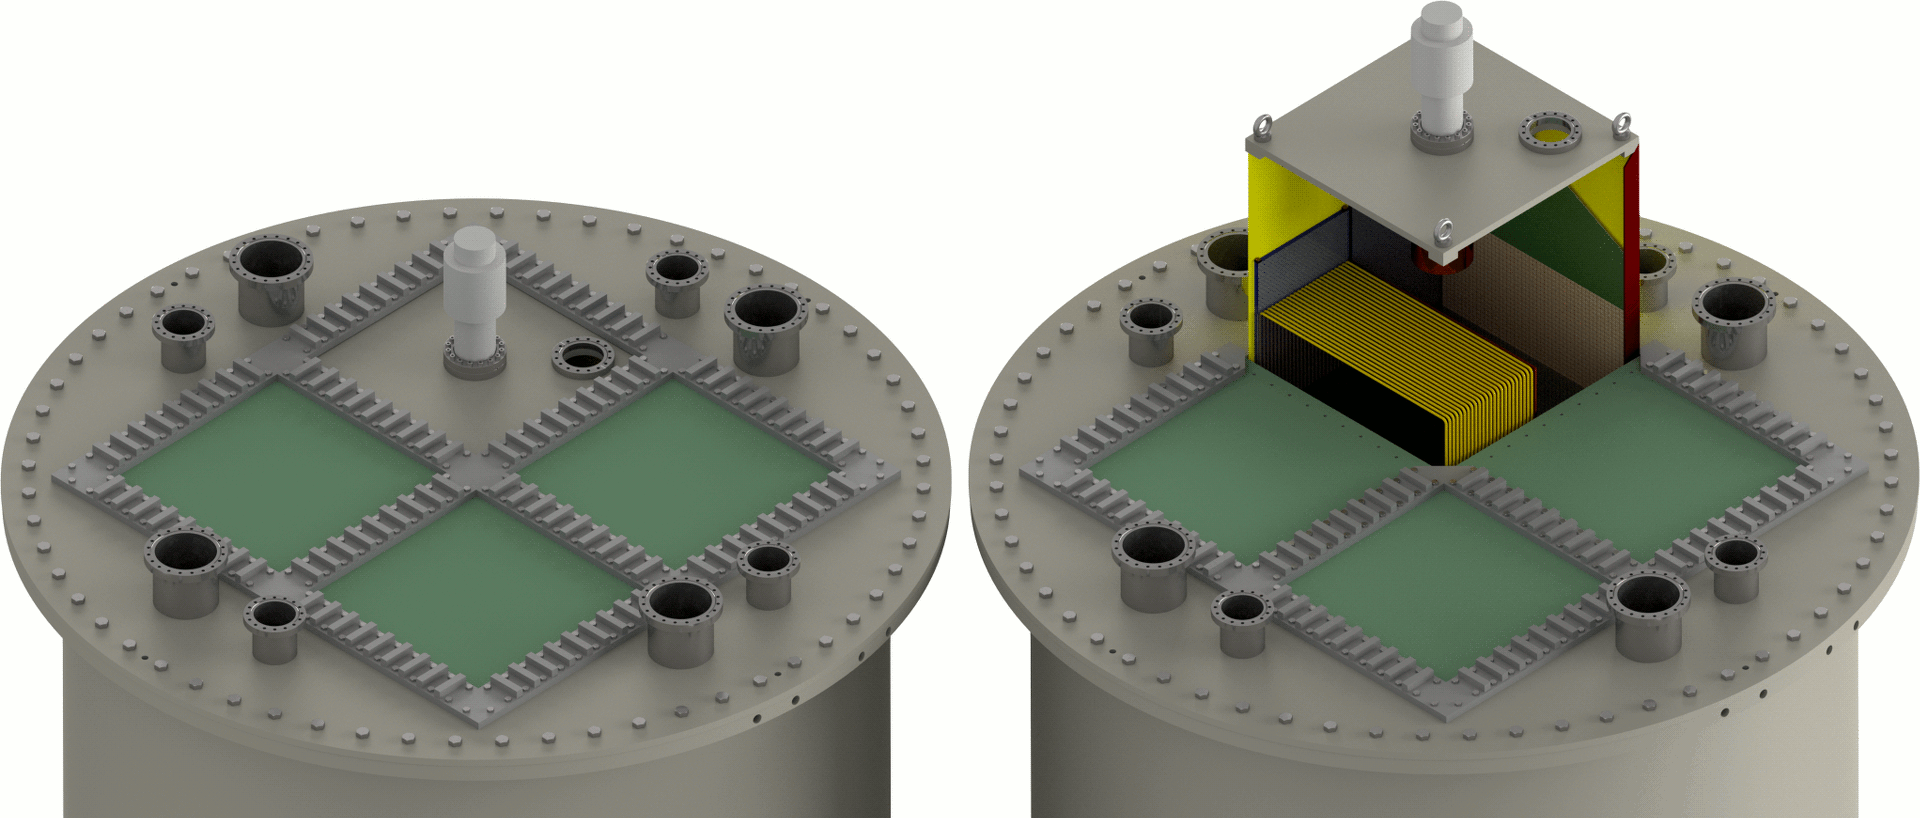
\includegraphics[width=\textwidth]{plots/DualBath.png}
\caption{Schematic view of the ArgonCube 2x2 demonstrator module. The four modules are visible, with one of them is partly extracted, on the right. This figure has been reproduced from Ref.~\cite{argoncube_loi}.}
\label{fig:2x2_extraction}
\end{figure}
Individual modules can be extracted or reinserted into a common LAr bath as needed, as is illustrated in Figure~\ref{fig:2x2_extraction}. Pressure inside the modules is kept close to the bath pressure putting almost no hydrostatic force on the module walls, which allows them to be thin, to minimize the inactive material in the walls. The purity of the LAr is maintained within each module independently, as will be described below. As a result, the argon surrounding the modules needs not meet as stringent purity requirements as the argon inside. Under normal operation conditions all modules are inserted with only clearance distances between modules. Cooling power to the bath is supplied by cryocoolers located in unistrumented volumes at the side of the detector called service volumes.

\begin{figure}[tbp]
  \centering
  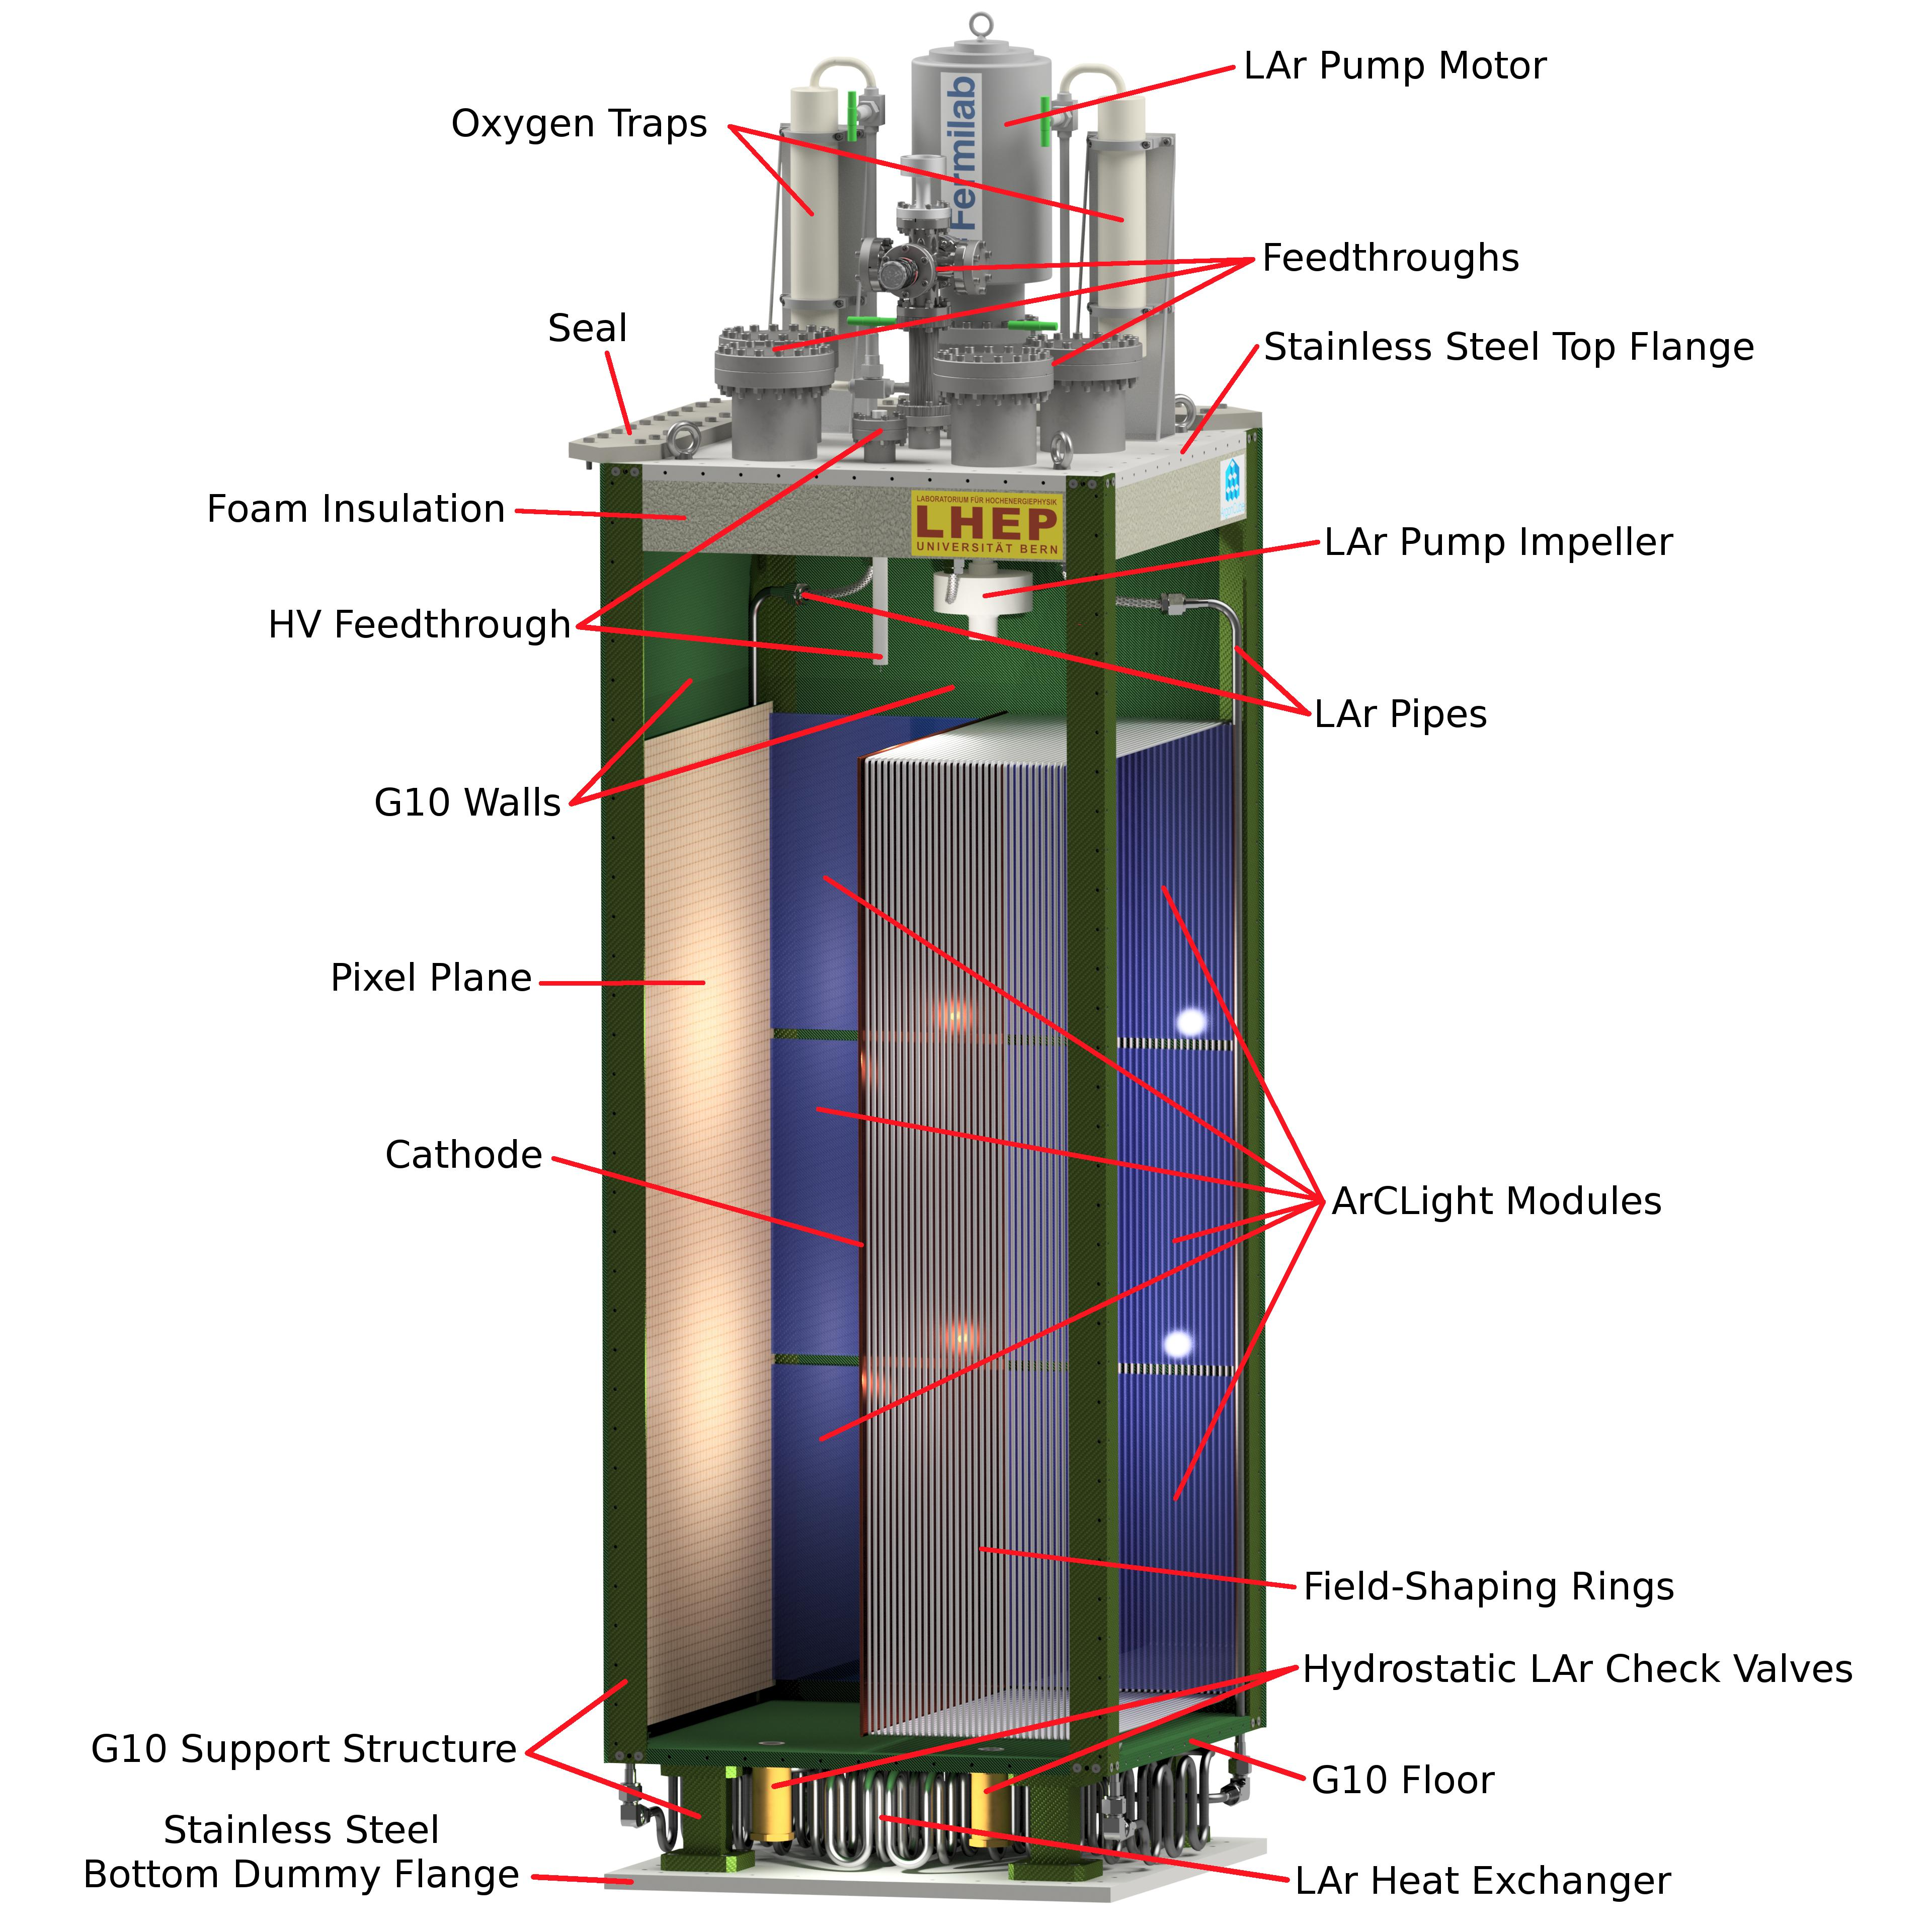
\includegraphics[width=0.8\textwidth]{plots/Normal-Module-4K_labelled}
  \caption[ArgonCube module engineering drawing]{Cutaway drawing of a \SI{0.67 x 0.67 x 1.81}{\metre} ArgonCube module for the $2\times2$ module prototype. \todo{Remove field shaping rings, and put in resistive field shell. -- who?}}
  \label{fig:ac_module}
\end{figure}
A cutaway drawing of an individual module is shown in Figure~\ref{fig:ac_module}. The side walls of each module are made from \SI{1}{\centi\metre} G10 sheets, to which the resistive field shell is bonded \todo{James, help me!}. G10's electromagnetic radiation length ($X_{\mathrm{0}} = \SI{19.4}{\centi\metre}$) and hadronic interaction length ($\lambda_{\mathrm{int}} = \SI{53.1}{\centi\metre}$)~\cite{pdg_g10} are both comparable to LAr ($1.4\times10^{-1}$~m and $8.37\times10^{-1}$~m respectively), making G10 structures in LAr almost transparent for passing particles, allowing for a performance comparable to a monolithic detector.

The key advantage of the modular design is that it does not require the high cathode voltage required for large monolithic detectors, and avoids the resulting stored energy problem. To minimize the voltage required, the drift field is applied along one of the short edges of a module. \todo{Isn't this also because reconstruction is harder if all of the tracks cross the cathode?} Additionally, the module is split into two TPCs by a central cathode, further reducing the required cathode potential by a factor of two. For the full size module footprint of \SI{1 x 1}{\metre} and an electric field of \SI{1}{\kilo\volt\per\centi\metre} a cathode potential of only \SI{50}{\kilo\volt} is required. \todo{And for the 2x2?}. Operating a LArTPC at this voltage is challenging but feasible without a prohibitive loss in active volume~\cite{argontube}. The key advantage of the modular design is that it does not require the high cathode voltage required for large monolithic detectors, and avoids the resulting stored energy problem. The HV is brought into the module using a commercially available feedthrough.\todo{Any other information required?}

During module insertion and extraction the argon flow is controlled by hydrostatic check valves located at the module bottom, which require a minimal differential pressure to open. Purity inside each module is maintained by means of continuous LAr recirculation through oxygen traps. Dirty argon is sucked in at the module top and then pushed through the oxygen traps, clean argon is first routed through a heat exchanger, located below the module inside the outer bath, for cooling and then re-enters the module at the bottom. For optimal heat transport the argon flow is directed along the cold electronics. To prevent dirty argon from the bath entering the modules their interior is held at a slight overpressure, just below the opening pressure of the check valves. \todo{James comment on whether each module has a pump etc}

ArgonCube offers true 3D tracking information using the LArPix pixelated charge readout and cryogenic electronics~\cite{larpix}, which are used to digitize the signals in the cold to avoid any channel multiplexing, and produce unambiguous 3D information. Pixelated anode planes are located on the two module walls parallel to the cathode. \todo{imfortant to state the dimensions?} The LArPix electronics, and a summary of their associated R\&D work, are described in Ref.~\cite{larpix}.

\begin{figure}[!ht]
\centering
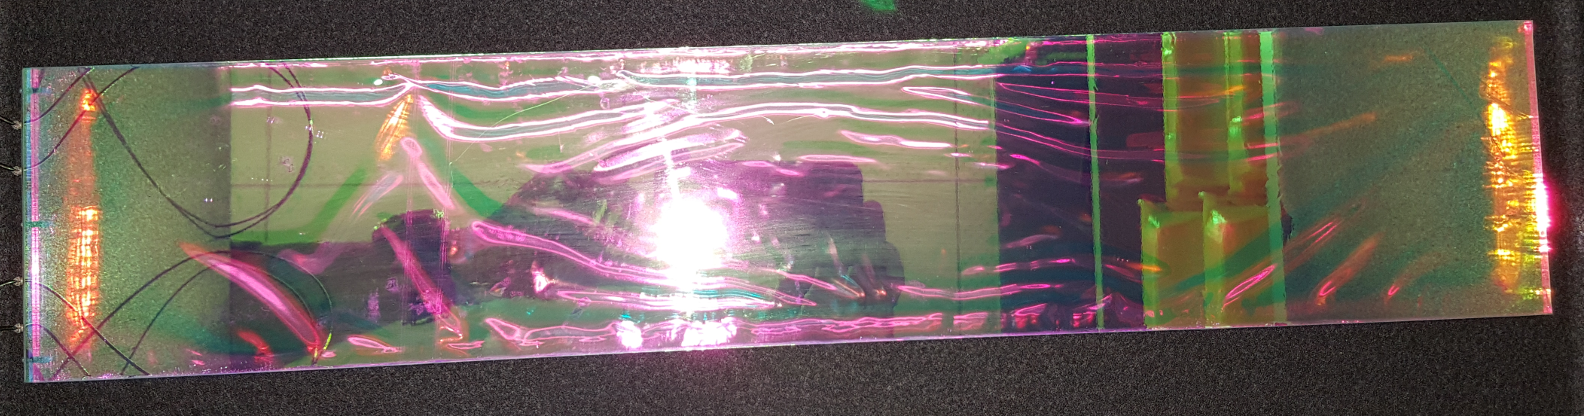
\includegraphics[width=0.75 \linewidth]{plots/1Film50x10.png}
\caption{A prototype ArgonCube light readout paddle built at the University of Bern. The paddle is 50~cm long and 10~cm wide, with four SiPMs coupled to one end. Reproduced from Ref.~\cite{argoncube_loi}.}
\label{fig:arclight}
\end{figure}
With LArPix, the reconstruction issues in a high rate environment are drastically simplified with respect to traditional projective wire readout TPCs, but in order to correctly reconstruct an event, scintillation signals need to be correctly matched to charge signals (flash matching). If these are correctly matched, the prompt scintillation light defines the time at which ionization electrons start to drift, and the time it takes to register charge on the anode plane along with the electric field strength allow give you enough information to reconstruct the third spatial co-ordinate (along the drift direction). In a modular detector, this problem can easily be made easier using an opaque cathode and module walls, which contains scintillation light to each TPC (half module), and effectively reduce the event pile-up. Furthermore, attenuation due to Rayleigh scattering,$6.6\times10^{-1}$~m, is much less of a problem than in large monolithic detectors. It is desirable to have a large area photon detection system to maximize the utility of scintillation light signals in the detector. However, the downside to modularization is the dead regions between adjacent TPCs, which introduce gaps in the reconstruction, so any light detection system must be compact. The solution pursued for the ArgonCube effort is ArCLight~\cite{arclight}, which is a very compact dielectric light trap that allows for light collection from a large area, inside high electric fields. An example ArCLight sheet is shown in Figure~\ref{fig:arclight}. These sheets are mounted on the walls of the module aligned with the drift direction, between the anode and the cathode. The additional dead volume of a few \si{\milli\metre} is similar to the one caused by the charge readout in the perpendicular direction.


\todo{James, can you comment on the 2x2 needs from the external nfrastructure point of view?}

\subsection{3DST}
\label{sec:3dst-design}
\todo{Chang Kee advised that there was no prototype expected on this timescale. Rewrite as a possible extension of the program if it becomes available.}

\subsection{HPTPC}
\label{sec:hptpc-design}
\todo{Alan said that he would talk with Jen and get back to us}

